% !TeX root = ../../main.tex
\subsection{Definición y propósito}\label{subsec:definicion-y-proposito}

\begin{definicion}
    El diseño de software consiste en crear un modelo que describa la arquitectura del sistema, los componentes que lo conforman, sus interfaces y las relaciones entre ellos.
    Se busca traducir los requisitos en una estructura organizada que guíe a la implementación.
\end{definicion}

\textbf{Propósitos principales:}
\begin{itemize}
    \item Facilitar la comunicación entre los participantes del proyecto.
    \item Servir de base para el análisis y la toma de decisiones.
    \item Identificar y gestionar las abstracciones clave del sistema.
    \item Promover la reutilización a gran escala (familias de productos).
\end{itemize}

\subsection{Importancia del diseño}\label{subsec:importancia-del-diseno}

Un buen diseño:
\begin{itemize}
    \item Permite traducir correctamente los requisitos en soluciones funcionales.
    \item Reduce el riesgo de errores, inestabilidad y dificultad de pruebas.
    \item Sienta las bases de la calidad del software.
\end{itemize}

\subsection{Atributos de calidad del software}\label{subsec:atributos-de-calidad-del-software}
\begin{itemize}
    \item \textbf{Funcionalidad:} capacidades del sistema, cobertura y seguridad.
    \item \textbf{Usabilidad:} facilidad de uso, estética, documentación.
    \item \textbf{Confiabilidad:} frecuencia y gravedad de fallos (MTBF, MTTR).
    \item \textbf{Rendimiento:} velocidad, tiempo de respuesta, uso de recursos.
    \item \textbf{Mantenibilidad:} facilidad para modificar, adaptar y probar.
\end{itemize}

\subsection{Conceptos clave del diseño}\label{subsec:conceptos-clave-del-diseno}

\begin{itemize}
    \item \textbf{Abstracción:} ocultar detalles para centrarse en lo esencial.
    \item \textbf{Arquitectura:} organización general del sistema y sus relaciones.
    \item \textbf{Patrones de diseño:} soluciones reutilizables a problemas comunes.
    \item \textbf{División de problemas:} estrategia de \textquote{divide y vencerás}.
    \item \textbf{Modularidad:} división del software en componentes independientes.
    \item \textbf{Ocultamiento de información:} cada módulo expone solo lo necesario.
    \item \textbf{Independencia funcional:} cada módulo resuelve tareas bien definidas.
    \item \textbf{Cohesión y acoplamiento:} coherencia interna y dependencia entre módulos.
    \item \textbf{Rediseño:} mejora estructural sin alterar funcionalidad.
\end{itemize}

\subsection{Clases de diseño}\label{subsec:clases-de-diseno}

\begin{itemize}
    \item \textbf{Interfaz de usuario:} elementos visibles e interactivos.
    \item \textbf{Dominio de negocio:} lógica y entidades principales.
    \item \textbf{Procesos:} gestión de tareas o flujos.
    Abstracciones de alto nivel que definen cómo se ejecutan las tareas.
    \item \textbf{Persistencia:} almacenamiento y recuperación de datos.
    \item \textbf{Sistema:} gestión de la infraestructura software.
\end{itemize}

\subsection{Elementos del modelo de diseño}\label{subsec:elementos-del-modelo-de-diseno}

\begin{itemize}
    \item \textbf{Diseño de datos:} organización de estructuras y bases de datos.
    \item \textbf{Diseño arquitectónico:} definición de subsistemas.
    \item \textbf{Diseño de interfaces:} entre componentes, usuarios y otros sistemas.
    \item \textbf{Diseño de componentes:} estructuras internas, algoritmos, interfaces.
    \item \textbf{Diseño de despliegue:} mapeo lógico-físico (servidores, contenedores).
\end{itemize}

\subsection{Diseño de arquitectura y patrones}\label{subsec:diseno-de-arquitectura-y-patrones}

\begin{definicion}
    \textbf{Arquitectura:}
    Estructura o estructuras del sistema, lo que comprende a los
    componentes del software, sus propiedades externas visibles y las
    relaciones entre ellos.
\end{definicion}

\subsubsection{MVC (Modelo-Vista-Controlador)}
\begin{minipage}{0.65\textwidth}
    \begin{itemize}
        \item \textbf{Modelo}: Datos y lógica negocio
        \item \textbf{Vista}: Interfaz usuario (presentación)
        \item \textbf{Controlador}: Mediador (recibe inputs, actualiza modelo)
        \item \textbf{Flujo}:
        \begin{enumerate}
            \item Usuario → Acción → Controlador
            \item Controlador → Actualiza Modelo
            \item Modelo → Notifica → Vista
            \item Vista → Renderiza → Usuario
        \end{enumerate}
        \item \textbf{Ventajas}: Separación preocupaciones, escalable
        \item \textbf{Uso}: Aplicaciones con UI compleja
    \end{itemize}
\end{minipage}
\hfill
\begin{minipage}{0.5\textwidth}
    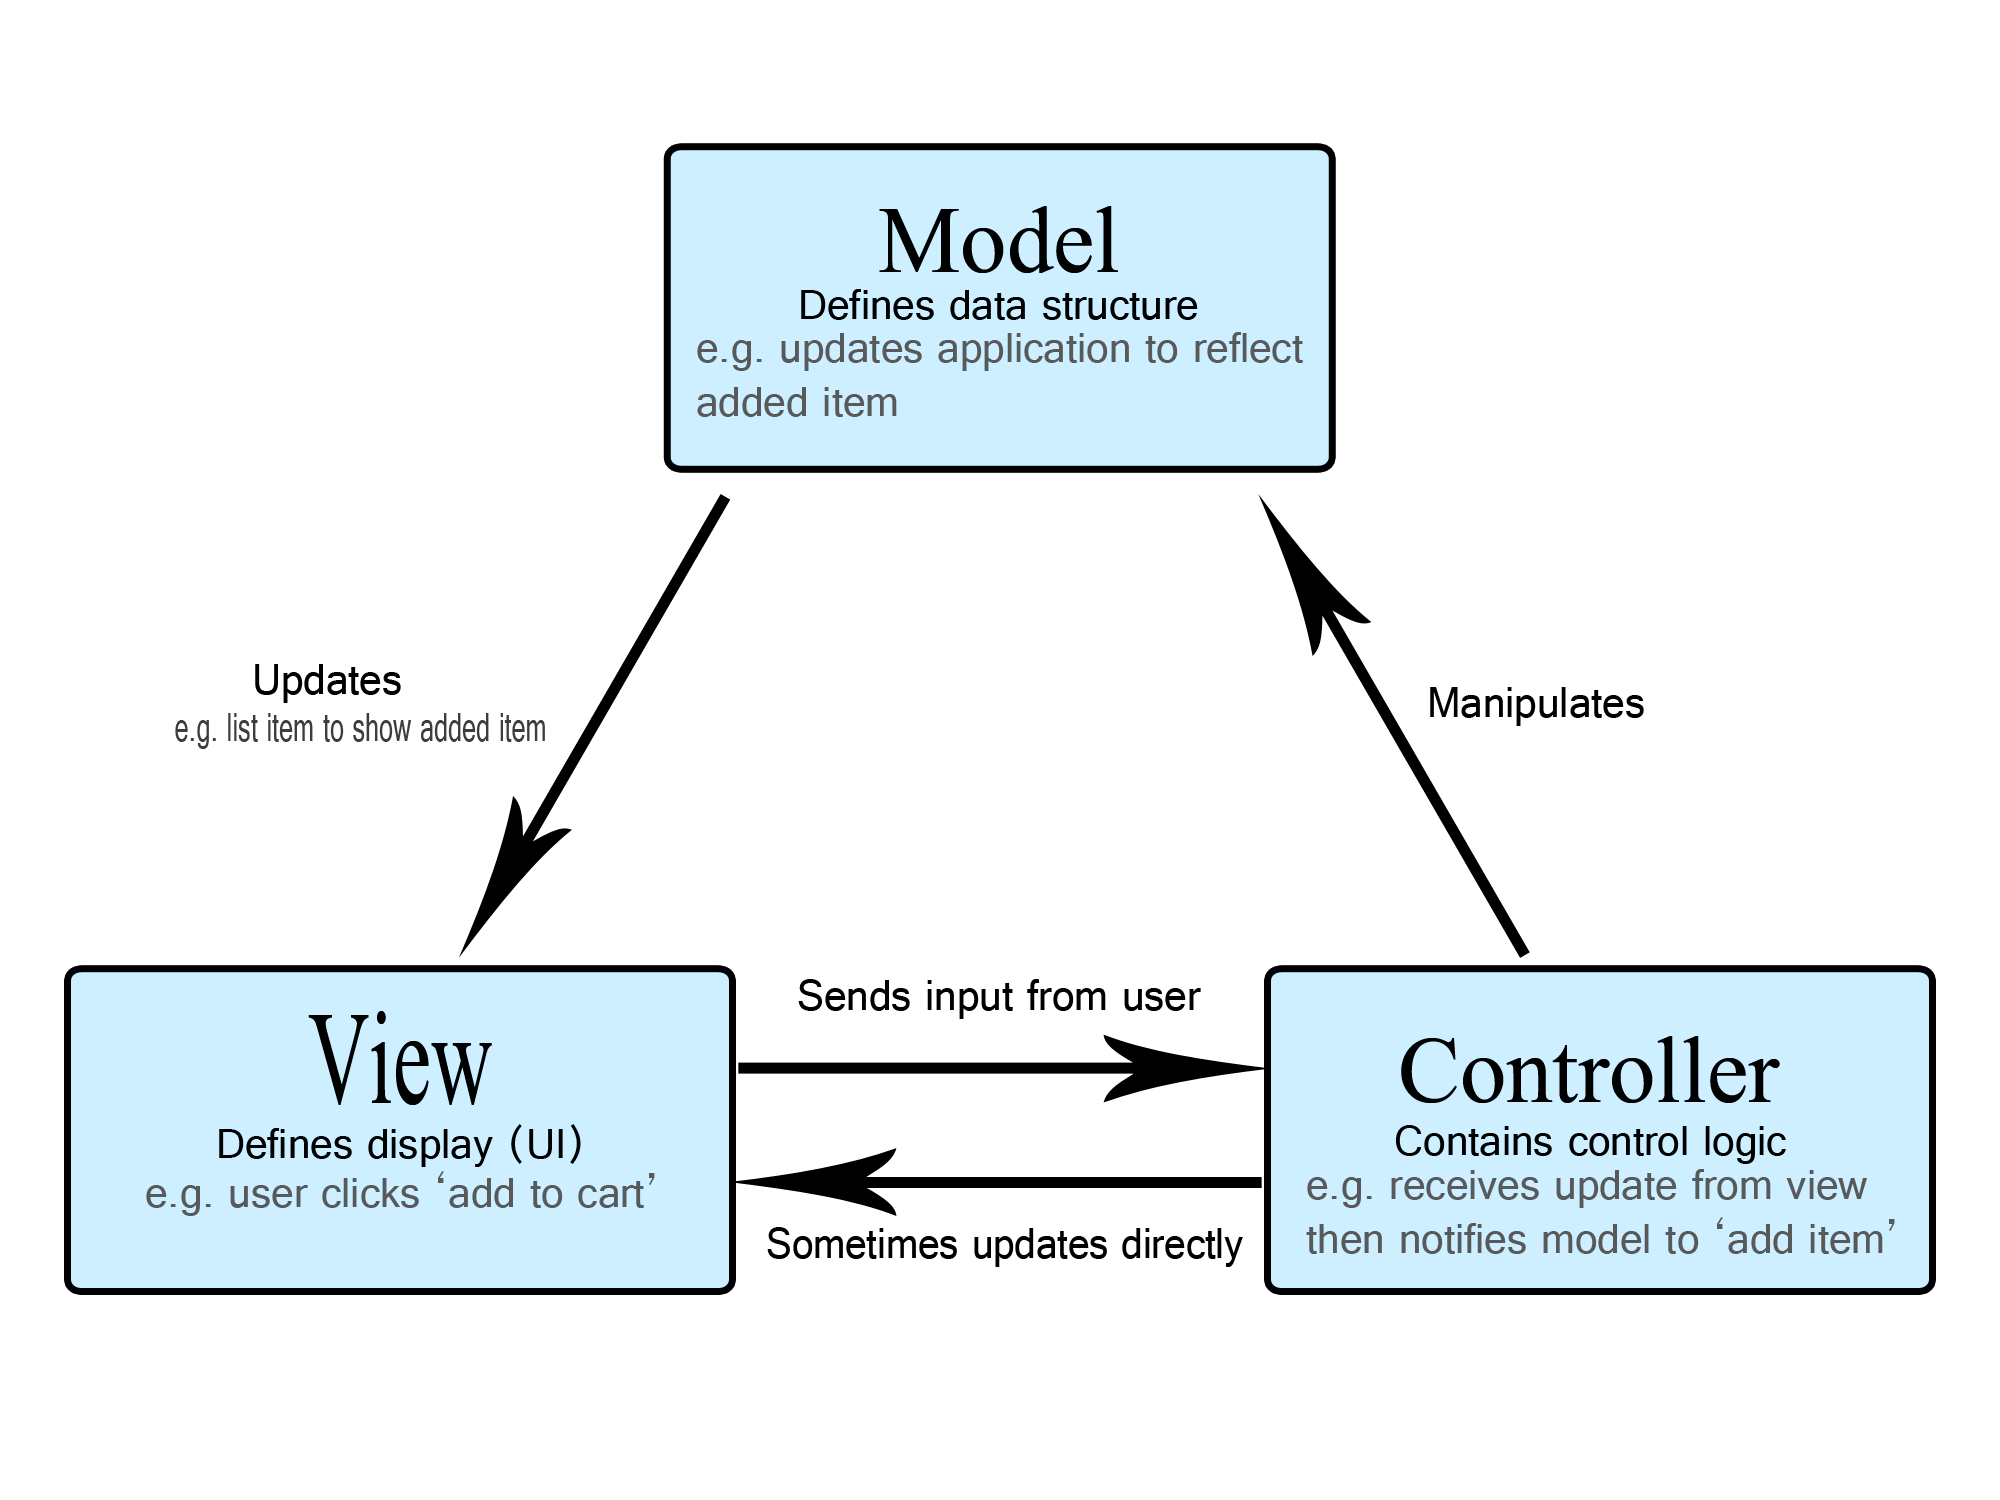
\includegraphics[width=\linewidth]{imagenes/model-view-controller-light-blue}
\end{minipage}

\subsubsection{SOA (Arquitectura Orientada a Servicios)}
\begin{itemize}
    \item Componentes autónomos (\textbf{Servicios})
    \item Comunicación mediante APIs
    \item \textbf{Niveles}:
    \begin{itemize}
        \item Integración
        \item Lógica negocio
        \item Acceso datos
    \end{itemize}
    \item \textbf{Ventajas}: Bajo acoplamiento, escalabilidad horizontal
    \item \textbf{Desafío}: Complejidad integración
\end{itemize}
\hfill
\begin{minipage}{0.5\textwidth}
    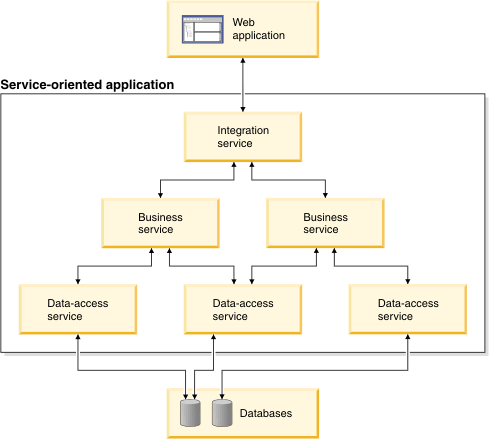
\includegraphics[width=\linewidth]{imagenes/soa}
\end{minipage}

\subsubsection{EDA (Arquitectura Dirigida por Eventos)}
\begin{itemize}
    \item Componentes: \textbf{Productores} (generan eventos) y \textbf{Consumidores} (reaccionan)
    \item Comunicación asíncrona mediante eventos
    \item \textbf{Ventajas}: Escalabilidad, tiempo real
    \item \textbf{Uso}: Sistemas IoT, alta concurrencia
\end{itemize}
\begin{minipage}{0.5\textwidth}
    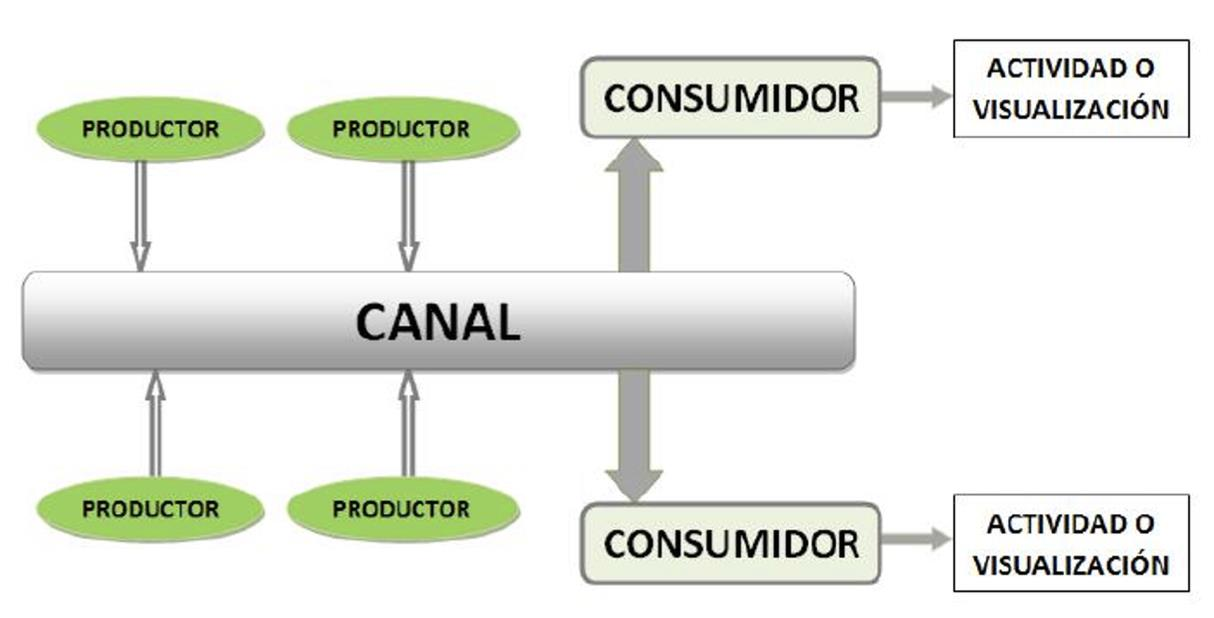
\includegraphics[width=\linewidth]{imagenes/eda}
\end{minipage}

\subsubsection{Otros Patrones}
\begin{itemize}
    \item \textbf{Layered}: Organización en capas (presentación, negocio, datos)
    \item \textbf{Microservicios}: SOA con servicios más pequeños y especializados
    \item \textbf{Workflow}: Orquestación de procesos secuenciales
\end{itemize}

\subsection{Diseño de interfaz de usuario}\label{subsec:diseno-de-interfaz-de-usuario}

\begin{definicion}
    El diseño de interfaz de usuario (UI) es el proceso de crear componentes visuales y funcionales que permiten a los usuarios interactuar con el software.
    Busca optimizar la experiencia del usuario (UX) y facilitar la usabilidad.
    Recoge los datos del subsistema de lógica de negocio
    para mostrarla.
    Reenvía las interacciones del usuario al subsistema de lógica de negocio para su procesado.
\end{definicion}

\textbf{Tipos:} GUI (gráfica), TUI (texto), VUI (voz).

\textbf{Aspectos clave:}
\begin{itemize}
    \item Usabilidad (eficiencia, satisfacción, accesibilidad).
    \item Personas: perfiles de usuario y escenarios de uso.
    \item Aspectos: claridad, tiempo de respuesta, ayuda, errores, internacionalización.
    \item Principios: familiaridad, uniformidad, recuperabilidad, diversidad.
\end{itemize}

\subsubsection{Principio de familiaridad en el diseño de interfaces}


El principio de familiaridad busca que el usuario se sienta cómodo desde el primer uso de la interfaz, aprovechando convenciones conocidas o comportamientos esperados.
Esto facilita la adopción del sistema, mejora la usabilidad y reduce la curva de aprendizaje.


Algunas técnicas comunes asociadas a este principio son:


\begin{itemize}

    \item \textbf{Lazy registration:} permite que los usuarios accedan parcialmente a la funcionalidad sin necesidad de autenticarse inicialmente.
    Solo cuando la acción lo requiere, se solicita el registro o inicio de sesión.

    \begin{itemize}

        \item \textbf{Propósito:} evitar fricción en el primer uso y fomentar la adopción.

    \end{itemize}
    \item \textbf{Breadcrumbs (migas de pan):} muestran la ruta de navegación desde la página principal hasta la ubicación actual.
    \begin{itemize}
        \item \textbf{Propósito:} permitir al usuario orientarse y volver atrás con facilidad.
    \end{itemize}

    \item \textbf{Hover control:} oculta información secundaria y solo la muestra cuando el usuario sitúa el cursor encima del elemento.
    \begin{itemize}
        \item \textbf{Propósito:} reducir la carga cognitiva y evitar distracciones.
    \end{itemize}

    \item \textbf{Search filters:} ofrece comandos o filtros de búsqueda predeterminados o sugerencias.
    \begin{itemize}
        \item \textbf{Propósito:} facilitar la exploración y ayudar al usuario a reconocer lo relevante.
    \end{itemize}

    \item \textbf{Carrito de la compra (e-commerce):} el carrito es accesible desde cualquier sección del sitio.
    \begin{itemize}
        \item \textbf{Propósito:} mejorar la experiencia de compra y aumentar la conversión.
    \end{itemize}
\end{itemize}

\subsubsection{Proceso de diseño de interfaz de usuario}

\begin{enumerate}
    \item Comprensión de actividades del usuario.
    \item Arquitectura de información.
    \item Prototipado de baja fidelidad.
    \item Pruebas de usabilidad.
    \item Diseño final (alta fidelidad, posible código).
\end{enumerate}

\subsection{Componentes}\label{subsec:componentes}

\begin{definicion}
    \textbf{Componentes:} unidades reutilizables del sistema que encapsulan funcionalidad.
    Cada componente tiene una interfaz bien definida y puede interactuar con otros componentes.
    Los componentes pueden ser independientes o formar parte de un subsistema mayor.
\end{definicion}

\subsubsection{Identificación de componentes:}


La correcta identificación de componentes es fundamental para lograr un diseño robusto, modular y mantenible.
Se deben tener en cuenta los siguientes criterios:


\begin{itemize}

    \item \textbf{Relación directa con los requisitos:} cada componente debe corresponderse con una funcionalidad significativa descrita en los requisitos del sistema.

    \item \textbf{Agrupación lógica:} las responsabilidades del componente deben estar relacionadas funcional o temáticamente.

    \item \textbf{Fronteras bien definidas:} cada componente debe tener una interfaz clara y estable que delimite lo que ofrece al resto del sistema.

    \item \textbf{Bajo acoplamiento:} los componentes deben minimizar sus dependencias mutuas, de modo que un cambio en uno no afecte a los demás.

    \item \textbf{Alta cohesión:} todas las funciones internas del componente deben estar fuertemente relacionadas y contribuir a un único propósito.

    \item \textbf{Reutilización potencial:} debe evaluarse si el componente puede ser útil en otros proyectos o contextos.

    \item \textbf{Autonomía en el despliegue:} en arquitecturas modernas (como microservicios), es deseable que cada componente pueda desplegarse y escalarse de forma independiente.

\end{itemize}


\textbf{Ejemplos de componentes:}

\begin{itemize}

    \item Módulo de autenticación y gestión de usuarios.

    \item Servicio de generación de informes PDF\@.

    \item API de gestión de pedidos.

    \item Componente de acceso a base de datos (DAO).

    \item Microservicio de pagos.

\end{itemize}




\subsection{Revisión técnica formal}\label{subsec:revision-tecnica-formal}

\textbf{Objetivo:} detectar problemas antes de la implementación.

\textbf{Participantes:} equipo de desarrollo.

\textbf{Evaluación de:} mantenibilidad, seguridad, disponibilidad, rendimiento, funcionalidad, usabilidad, coste.